\section{Revisão da Literatura}

O livro escrito por \citeauthor{BookIA} \cite{BookIA} apresenta todos os conceitos necessários para se iniciar na área de inteligência artificial (IA).
Modelos de IA são pensados desde os primórdios da computação. Sempre foi almejado uma forma de se construir um algoritmo
que se auto-modelasse dependendo do problema, para ter a melhor solução possível,
e que conseguisse aumentar sua própria precisão apenas precisando de uma entrada maior, sem necessidade de modificação
do código em si.

Como citado por \citeauthor{AntColonyOptimization} \cite{AntColonyOptimization}, algoritmos baseados em colônias de formigas
e outros insetos, que possuem comportamentos parecidos, começaram a ser pensados ainda nos anos noventa. 
Percebendo detalhes na forma que formigas se organizam ao procurar melhores
caminhos para alcançar seus objetivos, inspirou vários pesquisadores a projetarem algoritmos que o imitem como forma
de otimização para a área de inteligência artificial.

Programar qualquer inteligência artificial possui o problema de sempre se preocupar com o tamanho da entrada para treinamento.
Uma IA que sempre precisa de grandes entradas para se ter bons resultados precisa de ter bom uso dos recursos disponíveis na máquina. 
Por conta disso, modelar esse programa aproveitando da computação paralela é fundamental para um bom uso desses recursos. 
A diferença de desempenho entre a versão sequencial para a versão paralela é tão significativo que projetar os algoritmos 
já pensando em torná-los paralelos pode fazer total diferença \cite{SequentialVSParallel}.

Como apresentado por \citeauthor{ParallelComputingCUDA}, vários problemas computacionais podem ser otimizados em GPUs.
O uso de CUDA para programação paralela de quantidades massivas de dados se torna extremamente necessária, uma vez que
placas de vídeo da Nvidia podem chegar a ser até 250 vezes mais rápida do que uma versão paralela em CPU Intel \cite{ParallelComputingCUDA}. 
Placas de vídeo possuem grande capacidade de calcular grandes quantidades de dados simultaneamente e inteligência artificial 
é uma aplicação que encaixa perfeitamente nesse propósito.

Muitos autores gostam de apontar como algumas linguaguens de programação são mais eficientes que outras 
quando testadas sobre alguns parâmetros.
No artigo \citetitle{C++vsPython} de \citeauthor{C++vsPython}, mostra-se como a diferença na escolha das ferramentas
usadas durante a construção de um \emph{software} tem grandes impactos no desempenho final de uma aplicação como
mostrado na figura \ref{fig:comparisonMemorycppvspython}.

\begin{figure}[!ht]
    \centering
    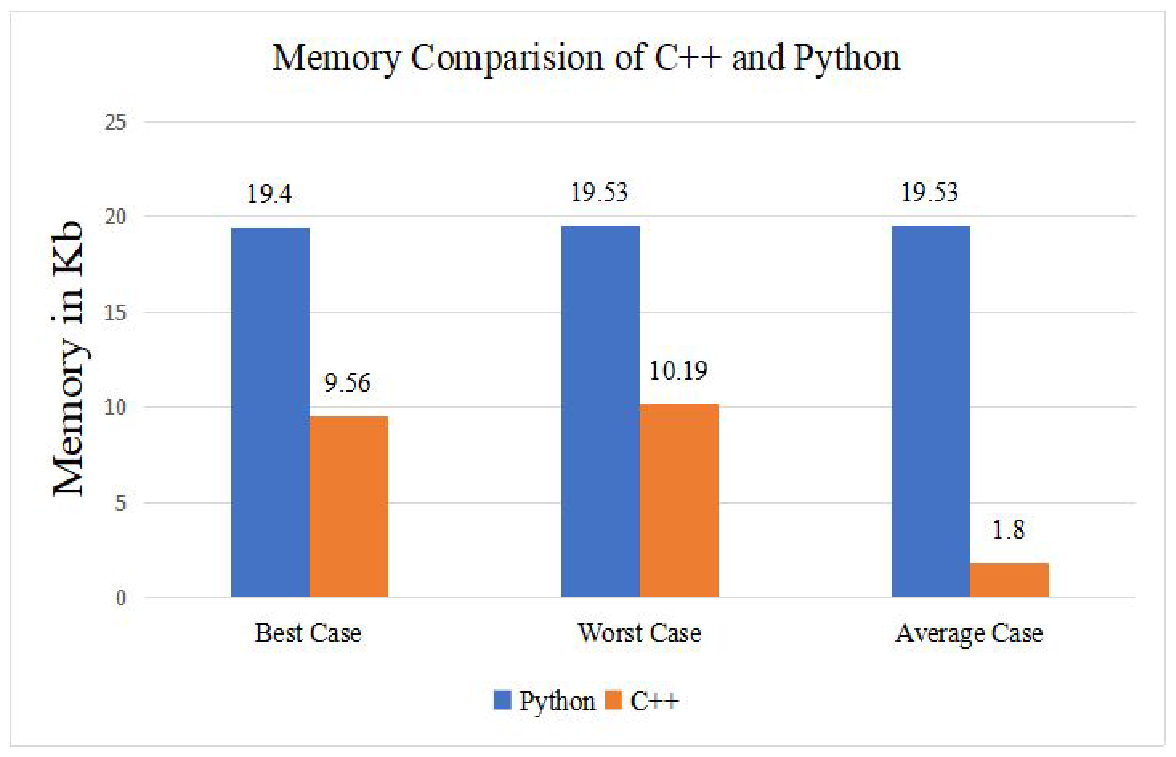
\includegraphics[width=0.5\textwidth]{ComparisonofMemoryConsumptionofSearchingAlgorithm.png}
    \caption[a]{Comparação do uso de memória em um algoritmo de busca\footnotemark.}
    \label{fig:comparisonMemorycppvspython}
\end{figure}

\footnotetext{Retirado do artigo: \citetitle{C++vsPython}.}

O uso de memória é extremamente importante de ser pensado quando se trata de um contexto de treinamento
de IA. O tempo de execução também é de suma importância de ser calculado, uma vez que teremos sempre 
grandes entradas para trabalhar. Pode-se ver na figura \ref{fig:speedcppvspython} a diferença de performance
entre ambas as línguas.

\begin{figure}[!ht]
    \centering
    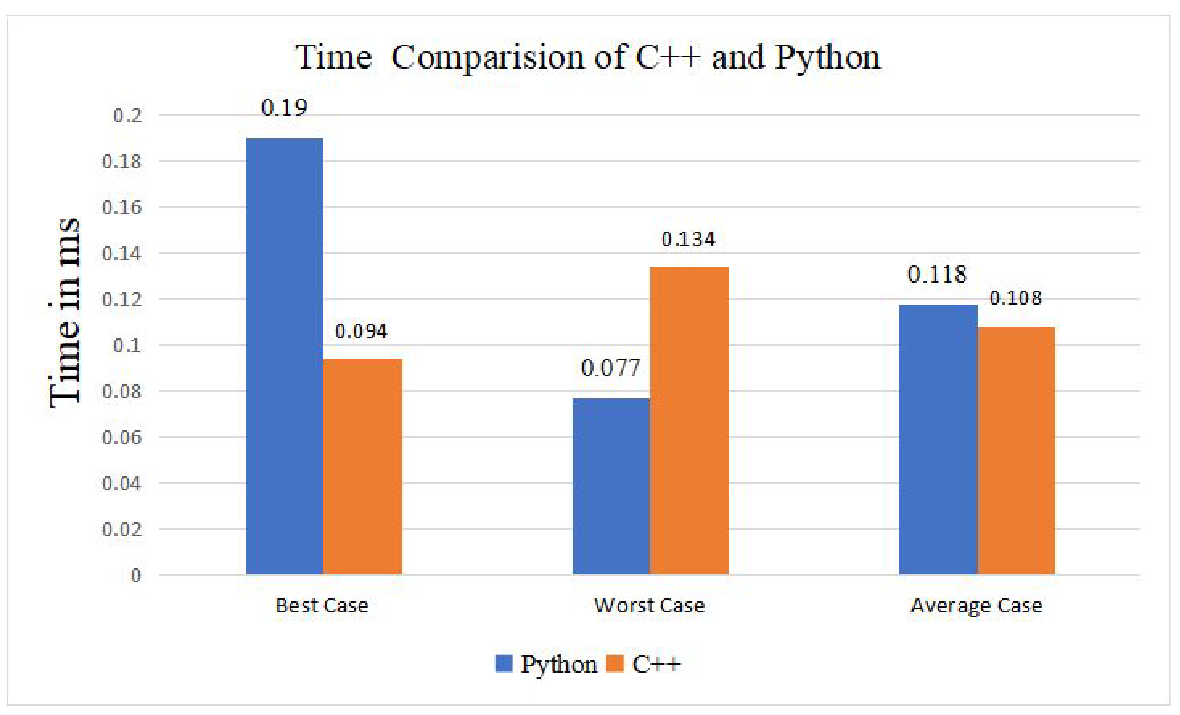
\includegraphics[width=0.5\textwidth]{ComparisonofTimeUtilizationofSearchingAlgorithm.png}
    \caption[a]{Comparação do tempo de execução de um algoritmo de busca de forma sequencial\footnotemark.}
    \label{fig:speedcppvspython}
\end{figure}

\footnotetext{Retirado do artigo: \citetitle{C++vsPython}.}

É notório que a linguagem de programação Python ficou atrás da linguagem C++ nesses parâmetros medidos. 
A primeira é consideravelmente mais simples de usar e ensinar para novos programadores \cite{C++vsPython}. 
Com isso em mente, o pesquisador \citeauthor{HPC_Python} apresentou em seu artigo \citetitle{HPC_Python},
como Python se tornou a língua favorita para os professores ensinarem e sua imensa utilidade na área científica. 
Por conta de sua facilidade de uso, houve grande atenção da comunidade para aumentar o desempenho dessa língua, até
que fique competitiva com o C++.

Trabalhos foram feitos para aumentar sua eficiência como citado por \citeauthor{JIT}, que em seu trabalho
para a IBM já em 2007, pensava em como aumentar o desempenho da linguagem de programação Java usando 
\emph{Just-in-Time Compiler}. Esse recurso permite que uma língua seja compilada para \emph{Bytecode}, o que
seria equivalente a uma lingua de programação intermediária entre o que a máquina consegue entender e o que o 
programador efetivamente escreveu. Isso permitia que um código não fosse completamente compilado para uma arquitetura
específica de processador, mas no momento de sua execução fosse modificado para o código de montagem de máquina
mais eficiente que estivesse disponível \cite{JIT}.

Considerando que Python é uma linguagem interpretada. Unir a ideia do \emph{JIT} que estava sendo empregada a 
vários anos no interpretador de Python poderia gerar bons resultados. O primeiro teste feito por \citeauthor{NumbaLLVMJIT}
apresentou ótimos resultados como mostrado na figura \ref{fig:numbavspythonsequencial}.

\begin{figure}[!ht]
    \centering
    \begin{tabular}{|c|c|c|}
        \hline
        Tamanho da Matriz & Numba & C \\
        \hline
        64 x 64 & 463x & 453x \\
        \hline
        128 x 128 & 454x & 407x \\
        \hline 
        256 x 256 & 280x & 263x \\
        \hline
        512 x 512 & 276x & 268x \\
        \hline
    \end{tabular}
    \caption[a]{Comparativo entre o tempo de execução do Numba e de um código em C para multiplicação de matrizes\footnotemark[3].}
    \label{fig:numbavspythonsequencial}
\end{figure}

% Aparece no final da página, não está relacionado com o texto que está sendo escrito em volta
\footnotetext[3]{Retirado do artigo: \citetitle{NumbaLLVMJIT}.}

Com esses resultados é possível comprovar que com as otimizações certas, pode-se tornar o Python tão performático quanto C++.
Muitas outras otimizações foram feitas para ter-se ainda mais desempenho como \emph{deferred loop specialization}, reescrita
das equações das matrizes e o uso de ferramentas para geração de \emph{Bytecode} otimizados com LLVM.

Algoritmos para seleção de melhor instância como o \emph{K-Means} sempre foram referência quando discute-se
sobre algoritmos de \emph{clusterização}. No artigo escrito por \citeauthor{KmeansAlgorithm} \cite{KmeansAlgorithm},
mostra-se como há várias implementações extremamente eficientes para esse algoritmo e como a ordem de complexidade
pode ser elevada, assim como mostrado na figura \ref{fig:complexitykmeans}.

\begin{figure}[!ht]
    \centering
    \begin{tabular}{|c|c|c|c|}
        \hline
        Complexidade & \emph{K-Means} & \emph{Constrained-K-Means} & \emph{X-Means} \\
        \hline 
        Tempo & $O(n^2)$ & $O(kn)$ & $O(n\log k_{max})$ \\
        \hline  
        Espaço & $O((n+k)d)$ & $O((n+k)d)$ & $O((n+k)d)$ \\
        \hline
    \end{tabular}
    \caption[a]{Complexidade de algumas implementações do \emph{K-Means}\footnotemark.}
    \label{fig:complexitykmeans}
\end{figure}

\footnotetext{Retirado do artigo: \citetitle{KmeansAlgorithm}.}